\documentclass[preprint]{elsarticle}
% 
% 
% 
\usepackage[a4paper, top=20mm, left =20mm, right =20mm ,bottom=20mm ]{geometry}
\usepackage{lineno}
\modulolinenumbers[1]
\journal{TRE}
\usepackage{graphicx}
\usepackage{ulem}
\usepackage{array}
\usepackage{epstopdf}
\usepackage{amstext}
\usepackage[utf8]{inputenc}
\usepackage[english]{babel}
\usepackage{amsfonts}
\usepackage{color}
\usepackage{amssymb}
\usepackage[citecolor=blue,linkcolor=blue,colorlinks=true]{hyperref}
\usepackage{multirow}
\usepackage{amsmath}
%\usepackage{lmodern}
%\usepackage{booktabs}
\usepackage{float}
\usepackage{tabularx}
\usepackage{geometry}
\usepackage{lscape}
\usepackage{longtable}
\usepackage{romannum}
\usepackage{makecell}
\usepackage{adjustbox}
\usepackage{lscape} 
%\usepackage{hyperref}

\usepackage{booktabs}

\usepackage{cleveref}
\usepackage{tablefootnote}
\crefformat{footnote}{#2\footnotemark[#1]#3}
\usepackage{blindtext}
\usepackage{algorithmicx,algpseudocode}
\usepackage[linesnumbered,ruled]{algorithm2e}
\usepackage{amsthm} % add by zhou
\newtheorem{theorem}{Theorem} % add by zhou
 
%\usepackage{longtable}
%\usepackage{natbib} 
%\usepackage[super,square]{natbib} 
\usepackage{longtable} 
\usepackage{float}
\usepackage{footnote}
\renewcommand{\thefootnote}{\arabic{footnote}}
%\pagenumbering{Roman} 
\pagenumbering{arabic} 
\newtheorem{definition}{Definition}
%\newcommand{\red}[1]{\textcolor{red}{#1}}
%%%%%%%%%%%%%%%%%%%%%%%
%% Elsevier bibliography styles
%%%%%%%%%%%%%%%%%%%%%%%
%% To change the style, put a % in front of the second line of the current style and
%% remove the % from the second line of the style you would like to use.
%%%%%%%%%%%%%%%%%%%%%%%
%% Numbered
%\bibliographystyle{model1-num-names}

%% Numbered without titles
%\bibliographystyle{model1a-num-names}

%% Harvard
% \bibliographystyle{model2-names.bst}\biboptions{authoryear}
%% Vancouver numbered
%\usepackage{numcompress}\bibliographystyle{model3-num-names}

%% Vancouver name/year
%\usepackage{numcompress}\bibliographystyle{model4-names}\biboptions{authoryear}

%% APA style
%\bibliographystyle{model5-names}
%\biboptions{authoryear}
%\bibliographystyle{apa}
%% AMA style
%\usepackage{numcompress}\bibliographystyle{model6-num-names}

%% `Elsevier LaTeX' style
%\bibliographystyle{elsarticle-num}
%%%%%%%%%%%%%%%%%%%%%%%
%\bibliographystyle{apalike}
\newlength\mylength
\renewcommand{\baselinestretch}{1.5}
% 
% 
% 
% 
% 
% 
% 
% 
% 
% 
% 
% 
% 

% 
% 
\begin{document}
\linenumbers
\begin{frontmatter}
    \title{An AI-based conceptual framework for port ranking}

    \author[1]{Yanjie Zhou}
    \author[1]{Xiaojin Wang}
    \author[2]{Zehao Qian}
    \author[1]{Tao Li}
    % 
    % 
    % 
    \cortext[cor1]{Author to whom correspondence should be addressed.}
    \address[1]{School of Management, Zhengzhou University,  China, 315100, China}
    \address[2]{Department of Nature Sciences, Durham University, DH1 3LE, UK}

    \begin{abstract}
    
        In this paper, i

    \end{abstract}
    \begin{keyword}

    \end{keyword}
\end{frontmatter}
% 
% 
% 
% 
% 
\section{Introduction}

\section{Port ranking}

\subsection{Container port}
\subsubsection{Seaport}

Seaports are often located on the coast, facing the ocean,with deep-water channels and large dock facilities,being used for maritime cargo transportation and ship docking. Seaports also provide cargo handling, warehousing and other related services, connecting the goods flow among countries and regions. Seaports can be connected to sea and air transport to work as a part of multimodal transportation. Seaports usually have great oceanic landscapes around, and could offer various amusement facilities, which will attract large visitors to come for vacations, ensuring them convenient and comfortable experiences. So, seaports could not only develop local economy in many aspects such as tourism, manufacturing and logistics, but also provide working opportunities. However, seaports may pollute the ocean by exhausting gas from ships, discharging wastewater, litter and so on.To ensure a sustainable development and protect marine ecosystem, seaports gradually pay attention to green development by lowering bad impacts on the environment around, such as encouraging ships to use clean and new energy, exhausting gas or wastewater after treatment,  building shore power facilities to attracting ships to use,establishing protected areas, etc.

\subsubsection{Dry port}

Dry ports are seated in inland areas, serving as cargo distribution centers, usually being far from seaports. It transports goods through railways or highways. Dry port provide similar logistics services as seaports,but it pay more attention to connecting railways and highways
But dry ports are lack in the aspects of tourism and entertainment.As for developing local economy, dry ports contribute the same as seaports and river ports, but in different way.

\subsubsection{River port}

River ports are typically situated in inland areas,with shallow-water channels and smaller dock facilities, serving the transportation of small ships and light cargo. River ports, connecting different regions through rivers, can also serve as cargo distribution centers and tourist attractions and places for leisure.River ports facilitate trades respectively. Due to the inland locations, dry ports have smaller affection on the ecological environment, but still need to contribute to protect their environment around.

\subsection{What is port ranking?}

Port ranking refers to the evaluation and ranking of ports around the world or within a specific area based on a series of indicators and data to measure how important and competitive they are in the field of international trade and shipping. These indicators and data usually include cargo throughput, container throughput, ship calls, port facilities,service levels and so on. Port ranking offers stakeholders such as shipping companies, consignors of cargo and governments a reference to estimate the competitiveness and reliability of ports and make  decisions correspondingly. The results of port ranking may vary because different methods and indicators might be used for assessing ports.

\subsection{Who cares about port ranking?}

Benefits of port ranking

\subsubsection{Port operator}

Ports at the top of port ranking of "Port cargo, container throughput" will attract more cargoes and containers. The higher the port ranking, the greater the operational capacity of the port is. So the port ranking helps more customers to send more cargoes to top ports.

Port ranking will encourage operators to allocate resources more rationally. The lastest port ranking of national port throughput from January to July 2023 shows that Shenzhen port dropped to rank 20 (chart 1). The main reason is that a large number of Asia-North America routes are suspended/cancelled, while Shenzhen Port focuses on US shipping line. To go higher on the ranking and increase container throughput at Shenzhen port, the port operator could transfer more manpower and material resources to support other busier routes

Port ranking makes the top ports more famous, which will attract more professional talents to work for the top ports, which could in return develop the ports better. Port operators will also try their best to improve work efficiency and quality.

\subsubsection{Shipping liner}

Port ranking is a comprehensive, authoritative and reliable reference list for shipping liners to select ports for shipping.
For example, through port ranking based on container port performance index, the shipping liner will find ports that save voyage time for liners, educe transportation costs, improve ship transportation capacity, and accelerate ship turnover.

What's more, small ports do not provide enough containers and cargoes. Ship companies could easily choose ports with greater cargo and container throughput as docking points to strive for supply of goods and improve space utilization.

\subsubsection{Government}

The port ranking is a reference for the government to do Infrastructure investments and resource allocation. The larger ports ranked in the top have greater driving capacity for the surrounding economy and higher demand for supporting facilities. The government can intuitively understand the local economic development by ports ranking and increase investments in infrastructure accordingly.

Port ranking can reflect the current situation of equipment and safety management in the port. The equipment in ports with large throughput has a large load. So, the government should supervise and strengthen the maintenance and repair of equipment in ports.

Port ranking can be a reference tool for formulating strategic planning and policies for ports. The top-ranked ports' operation, management, and construction modes are more representative and standardized. The government learned from top-ranked ports to formulate and improve the corresponding rules and systems.

\section{The conceptual model}
\begin{figure}[H]
    \centering
    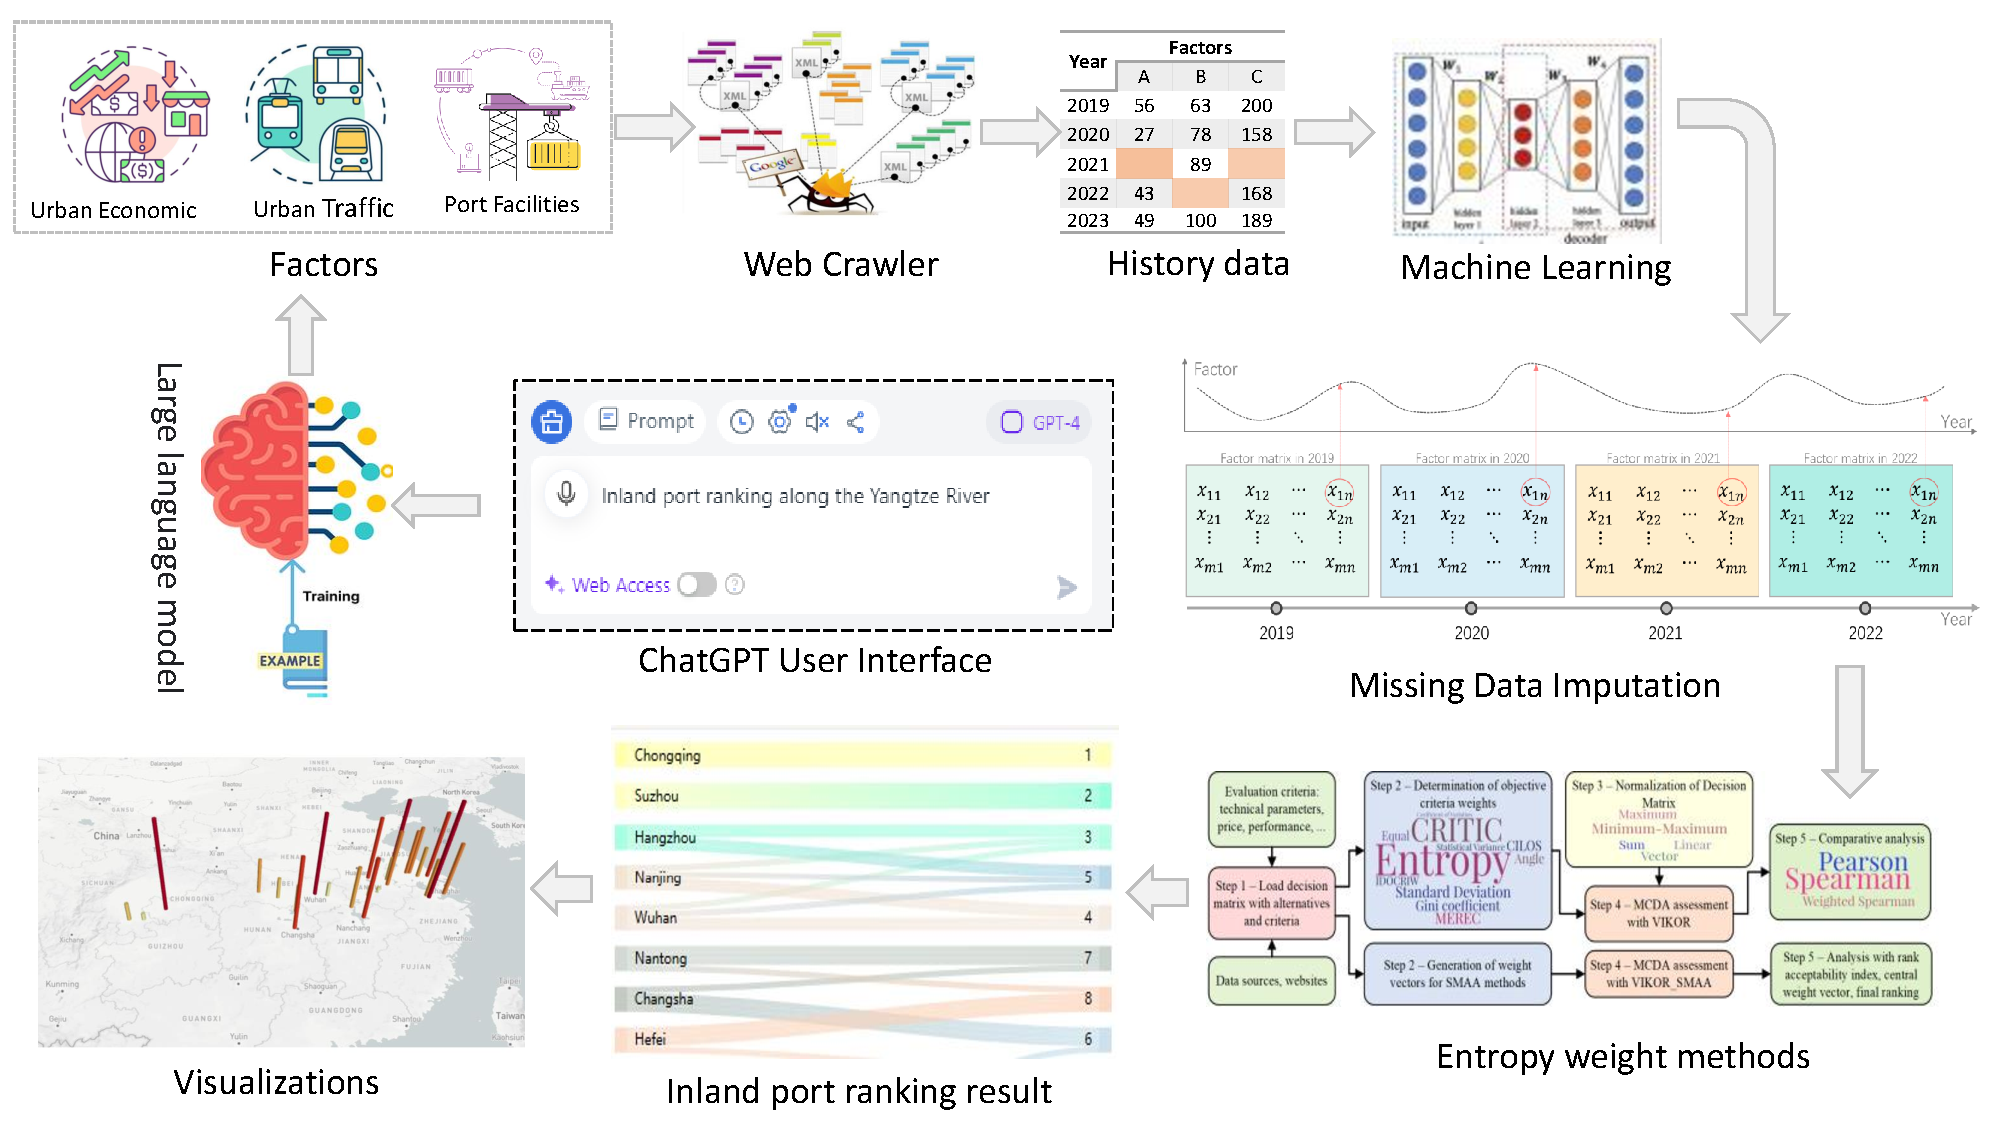
\includegraphics[width=1.0\textwidth]{pic/autoportranking.pdf}
    \caption{Caption}
    \label{fig:autoportranking}
\end{figure}
\subsection{Factors}
\begin{figure}
    \centering
    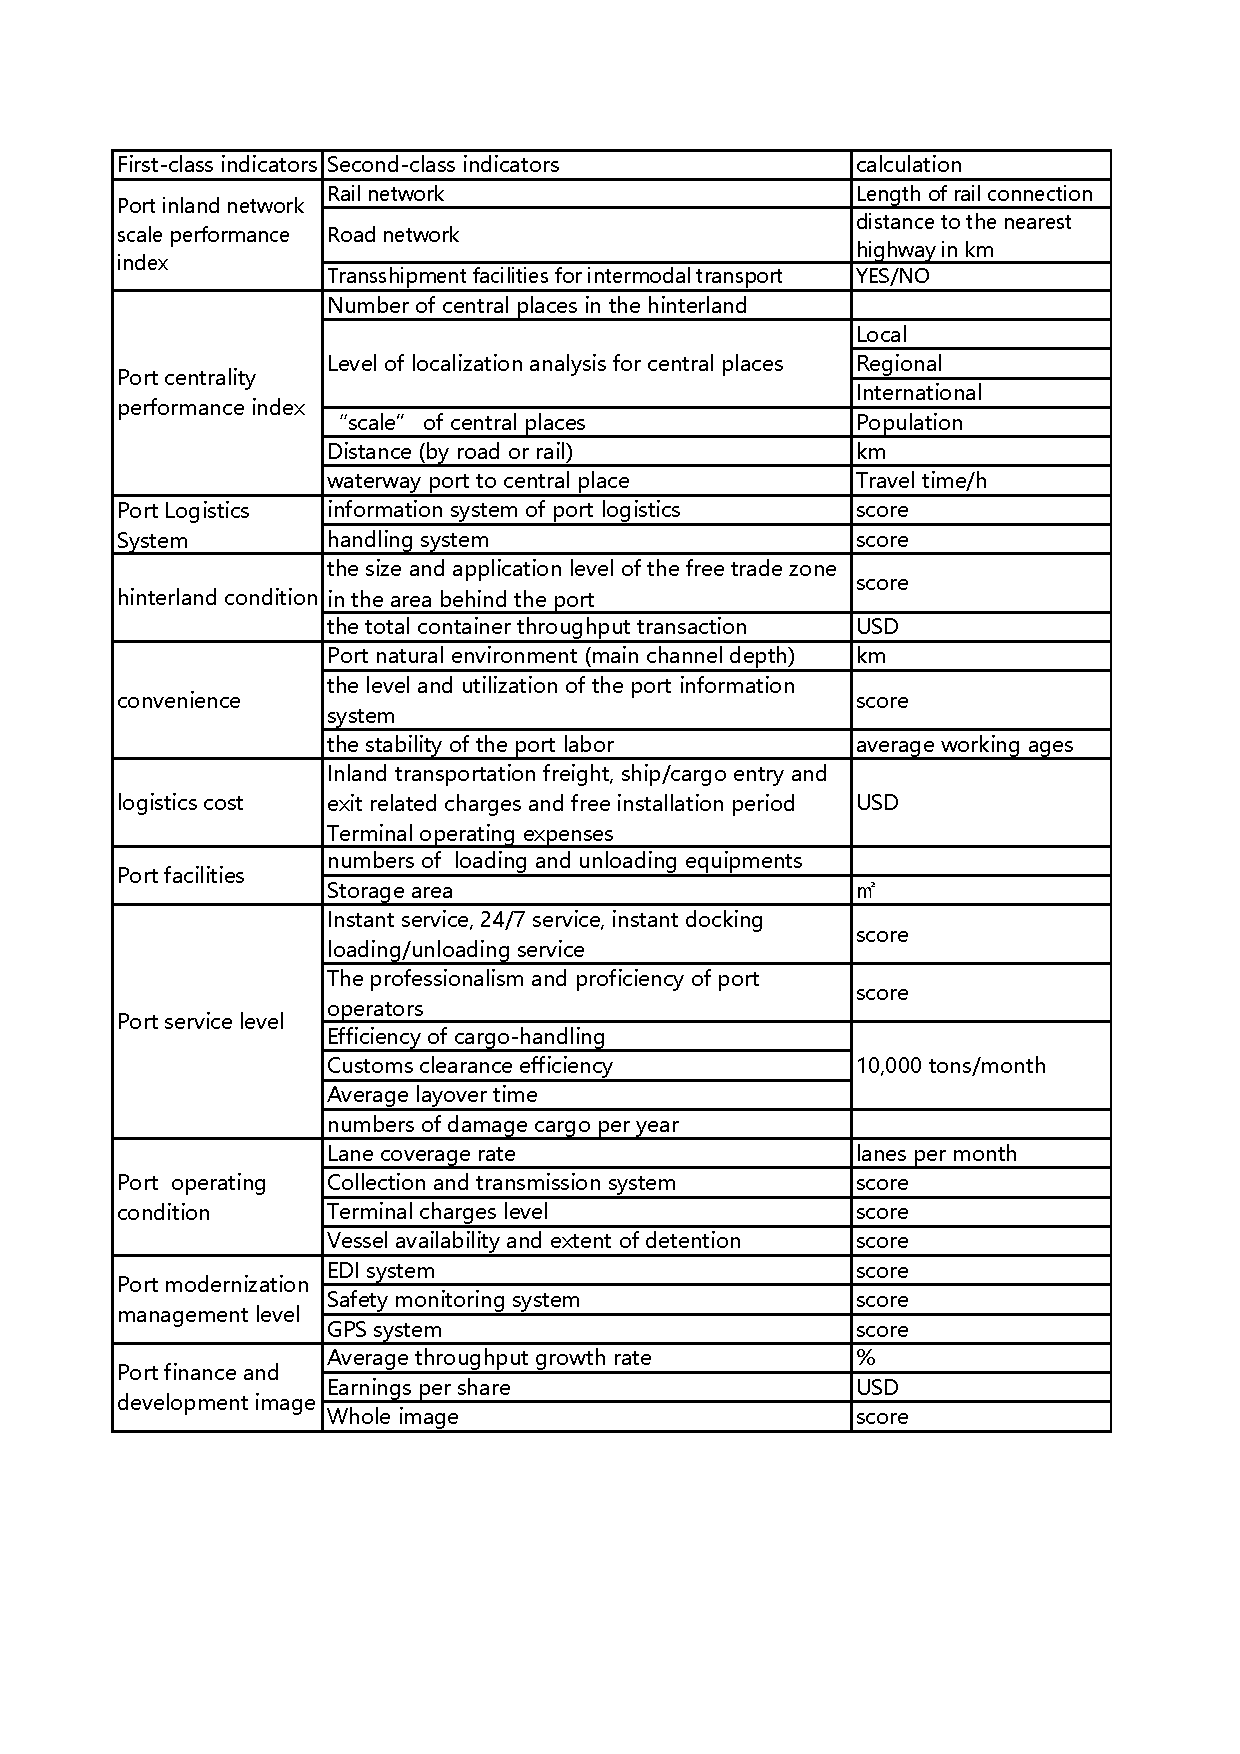
\includegraphics[width=1\linewidth]{pic/PortRankIndecator.pdf}
    \caption{Enter Caption}
    \label{fig:PortRankIndecator}
\end{figure}

Port ranking results that vary differently depend on network scales and centrality, and that the closer a port is to a main road or highway, the better the port development will be [O Dinu1 et al.,2016; Qing Liu,2022]. Three types of centrality measures,degree centrality, betweeness centrality and closeness centrality, are indicators to comprehensively evaluating the port importance[Chengpeng Wan et al., 2021]. The factors which affect port ranking result to different extent also include logistics cost, port service, hinterland condition and convenience level [Gitae Yeo et al., 2011]. Lu Shengrong and others build a port competitiveness evaluation index system of 6 first-class indicators: port natural environment, port infrastructures, Port service-level, port operating condition, port modernization management level, and port finance, development and image. When choosing ports to deploy the floating wind with lower cost, H. Díaz  and C. Guedes Soares find ports that near the wind farms and logistic centers is more efficiently exploit, and deep-water ports with large capacity is better[2023]. Adequate infrastructures,  frequency of ship visits and port location draw high attention from shipper when they select a port[CHINONYE UGBOMA et al., 2006]. Dan Zhao and others introduce green performance, port finance, market share and on-time delivery rate to evaluate a port[2021].

\subsection{Data collection}

To collect accurate data, a survey with is conducted for about 200 practitioners in the field of port operating and related. We also get data of factors from port management instituions, international trading organizations, shipping companies, port database and so on.

\begin{longtable}{
    >{\raggedright\arraybackslash}m{0.3\textwidth}
    >{\raggedright\arraybackslash}m{0.35\textwidth}
    >{\raggedright\arraybackslash}m{0.35\textwidth}
}
    \hline
    \textbf{Type}                     & \textbf{Advantages} & \textbf{Disadvantages} \\
    \hline
    \endfirsthead

    \hline
    \textbf{Type}                     & \textbf{Advantages} & \textbf{Disadvantages} \\
    \hline
    \endhead

    \hline
    \endfoot

    \hline
    Traditional Web Crawlers          &
    - Fast speed\newline
    - Low resource consumption\newline
    - Simple and easy to use          &
    - Poor flexibility\newline
    - Easily blocked by anti-crawling mechanisms                                     \\
    \hline
    Selenium-based Crawlers           &
    - Highly flexible\newline
    - Can handle complex scenarios    &
    - Slower speed\newline
    - High resource consumption\newline
    - High complexity                                                                \\
    \hline
    LLM-based Intelligent Crawlers    &
    - Strong understanding ability\newline
    - Strong adaptability\newline
    - Capable of complex interactions &
    - Potential speed limitations\newline
    - Resource-intensive\newline
    - Challenges in accuracy                                                         \\
    \hline
\end{longtable}

\subsection{Missing Data imputation}

In modern port management and Operation Research, the integrity and accuracy of data is very important. Effective data analysis can not only reveal the current state of port operation, but also predict future trends and potential problems. However, data loss is a common problem in data collection, which can be caused by a number of factors, including technical failures, recording errors or delayed information updates. The purpose of this paper is to explore and solve this challenge in order to enhance the understanding and application of port data.

Firstly, the data collected from the port were examined to identify the patterns and possible causes of missing data. On this basis, we will explore various strategies to deal with missing data to ensure the accuracy and reliability of the analysis results. We will focus in particular on two major approaches: Imputation and Deletion. The interpolation method aims at estimating missing values and filling data gaps with these estimates, while the deletion method is to remove data records containing missing values.

\textbf{Delete or Impute?} When deciding whether to delete or impute missing data, consider the proportion and pattern of missingness, the nature of the data, the requirements of the analysis method, and the purpose of the study. Deletion is suitable for small proportions of randomly missing data and when it won't introduce bias, while imputation is preferred for large proportions of missing data, non-random missingness, to maintain dataset size and integrity, and to retain critical information. The decision should balance the characteristics of the data, the reasons for missingness, and the objectives of the analysis. \cite{Jakobsen2017}

\subsubsection{Traditional Missing Data Imputation Methods}

\textbf{Mean/Median/Mode Imputation} \cite{Kleinbort2020} is a common and simple method where all missing values are replaced with the mean, median, or mode of the column. Although this approach is easy and fast, it has its drawbacks. It can skew the statistical nature of the data, underestimate variance, and distort histograms. This method is generally advisable only when data is missing completely at random (MCAR) or missing at random (MAR), but it is not suitable if data is missing not at random (MNAR)

\textbf{Multiple Imputation} \cite{Sterneb2393} \cite{Khan2020} involves creating multiple copies of the dataset, where missing values are replaced with imputed values based on their predictive distribution from observed data. This method uses standard statistical methods to fit models to each imputed dataset, and then averages the results to provide overall estimated associations. Multiple imputation, based on a Bayesian approach, accounts for all uncertainty in predicting missing values by introducing appropriate variability into the imputed values. It is essential in multiple imputation to model the distribution of each variable with missing values accurately. However, pitfalls can occur, such as omitting the outcome variable from the imputation process or dealing incorrectly with non-normally distributed variables. The validity of results from multiple imputation depends on careful and appropriate modeling.

\textbf{KNN and linear regression imputing} \cite{10.1371/journal.pone.0295632} \cite{articleLearnKNN} \cite{inproceedingsKNearest} \cite{Emmanuel2021}
% 
% 
% 

\subsubsection{Imputing Missing Data with Deep Learning and LLMs}
% 
% 
% 

The great potential of deep learning in imputation of missing values in data. In the field of port management, these methods can be used to process and analyze large amounts of complex data, such as cargo flows, vessel dynamics, weather conditions, and port operation efficiency. Data imputation using deep learning not only improves data completeness and accuracy, but also helps predict and optimize port operations, thereby improving efficiency and safety. \cite{9458712} \cite{wang2022deep} \cite{park2022longterm} \cite{camino2019improving}
% 
% 
% 
% 
% 

In order to overcome the challenge of missing values in port data, this study proposes a method to predict and interpolate these missing values using a pre-trained model Xi machine learning. We first use existing port data, including multi-dimensional information such as cargo throughput, vessel arrival frequency, weather conditions, and port facility usage, to train our machine Xi model. This data has been cleaned and preprocessed to ensure the quality of the data fed into the model.
We chose a machine Xi model suitable for working with time series data, such as long short-term memory networks (LSTMs) or gated recurrent units (GRUs), because port data often have significant time-dependent and seasonal characteristics. The training of the model was performed on a rich historical dataset containing complete and missing instances of data collected from normal operations. In this way, the model learns Xi complex patterns and associations in the data, which can be used to predict missing values.
% 
% 
% 
% 
% 

% \subsubsection{Fitting of missing data}

\subsection{Entropy weight method}

\subsection{Ranking result analysis}
\subsection{Visualization of results}
\section{Conclusions}
\bibliography{references}
\end{document}